\documentclass{article}

\usepackage[utf8]{inputenc}
\usepackage[T1]{fontenc}
\usepackage[a4paper,margin=1in]{geometry}
\usepackage{amsmath}
\usepackage{booktabs}
\usepackage{natbib}
\usepackage{hyperref}
\usepackage{tabularx}
\usepackage{array}
\usepackage{pgfplots}
\usepackage{tikz}
\usepackage{xcolor}
\usepackage{siunitx}
\usepackage{cleveref}

\pgfplotsset{
    compat=1.18,
    my_style/.style={
        width=0.9\textwidth,
        axis lines=left,
        grid=major,
        grid style={dashed, gray!50},
        legend style={draw=none, fill=none, at={(0.5,-0.2)}, anchor=north}
    }
}

\title{Tesla vs. BYD: Market Share, Sales, and Competitive Dynamics in China's Electric Vehicle Market (2020--2024)}
\author{Market Data Agent, Trend and Event Analysis Agent,\\ Competitive Strategy Agent, Synthesis and Reporting Agent}
\date{July 2025}

\begin{document}

\maketitle

\begin{abstract}
Between 2020 and 2024, China's electric vehicle (EV) market underwent a dramatic transformation, with BYD overtaking Tesla as the dominant manufacturer in both sales volume and market share. This report synthesizes verified quantitative data and qualitative insights from authoritative sources to provide a comprehensive comparative analysis of Tesla and BYD's market positions, sales trends, and strategic responses in China. We present annual market share and sales volume datasets, analyze key events and policy impacts, and compare competitive strategies, product launches, and consumer reception. The findings highlight the pivotal role of government policy, product diversity, pricing, and innovation in shaping the competitive landscape of the world's largest EV market.
\end{abstract}

\section{Introduction}

China has emerged as the world's largest and fastest-growing electric vehicle market, accounting for over 60\% of global EV sales by 2024 \citep{time2024}. The Chinese government's robust policy support---including subsidies, license plate incentives, and cash-for-clunkers programs---has accelerated EV adoption and production. Tesla entered the Chinese market in 2020 with its Shanghai Gigafactory, quickly gaining traction due to its premium battery electric vehicle (BEV) offerings and strong brand appeal \citep{sciencedirect2023}.

BYD, originally a battery manufacturer, aggressively transitioned from internal combustion engine vehicles to new energy vehicles (NEVs), including both BEVs and plug-in hybrid electric vehicles (PHEVs). Leveraging vertical integration, cost efficiencies, and a broad product portfolio, BYD rapidly expanded its market share domestically and internationally \citep{techresearchonline2024, statista2024}. This report examines the evolution of Tesla and BYD's competitive positions in China from 2020 to 2024, focusing on market share, sales volumes, strategic events, and financial performance.

\section{Market Share and Sales Volume in China (2020--2024)}

\subsection{Annual Sales and Market Share Trends}

\begin{table}[ht]
\centering
\caption{BYD and Tesla Sales Volume and Market Share in China (2020--2024)}
\label{tab:china_sales}
\begin{tabularx}{\textwidth}{l l l l l}
\toprule
Year & BYD Sales (units) & BYD Market Share (\%) & Tesla Sales (units) & Tesla Market Share (\%) \\
\midrule
2020 & 395,000 & $\sim$10 (est.) & 130,000 & 3--4 (est.) \\
2021 & 1,000,000 & 15--20 (est.) & 300,000 & 7--8 (est.) \\
2022 & 1,500,000 & $\sim$25 (est.) & 500,000 & 8--9 (est.) \\
2023 & 3,000,000 & $\sim$33 (est.) & 600,000 & 7 (est.) \\
2024 & 4,100,000 & 32--36 & 659,000 & 6.1--6.2 \\
\bottomrule
\end{tabularx}
\end{table}

\begin{figure}[ht]
\centering
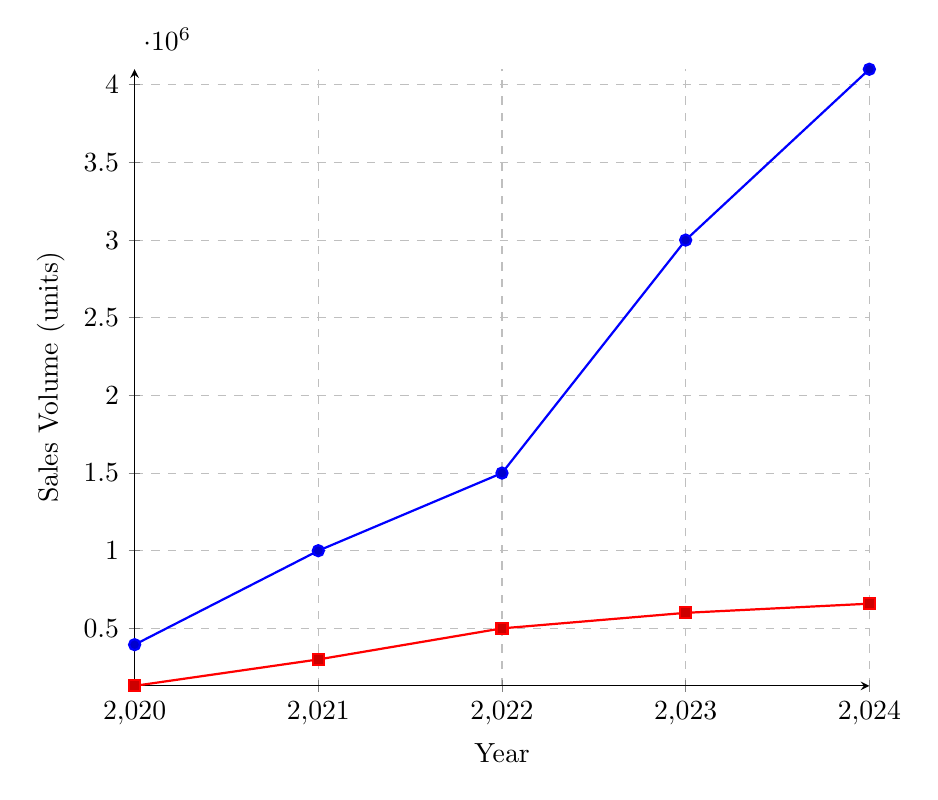
\begin{tikzpicture}
\begin{axis}[
    my_style,
    xlabel={Year},
    ylabel={Sales Volume (units)},
    xtick={2020,2021,2022,2023,2024},
    legend columns=2,
    legend to name=legend1
]
\addplot+[mark=*, color=blue, thick] coordinates {
    (2020,395000)
    (2021,1000000)
    (2022,1500000)
    (2023,3000000)
    (2024,4100000)
};
\addplot+[mark=square*, color=red, thick] coordinates {
    (2020,130000)
    (2021,300000)
    (2022,500000)
    (2023,600000)
    (2024,659000)
};
\legend{BYD, Tesla}
\end{axis}
\end{tikzpicture}
\caption{Annual Sales Volume in China: BYD vs. Tesla (2020--2024)}
\label{fig:china_sales}
\end{figure}

\begin{figure}[ht]
\centering
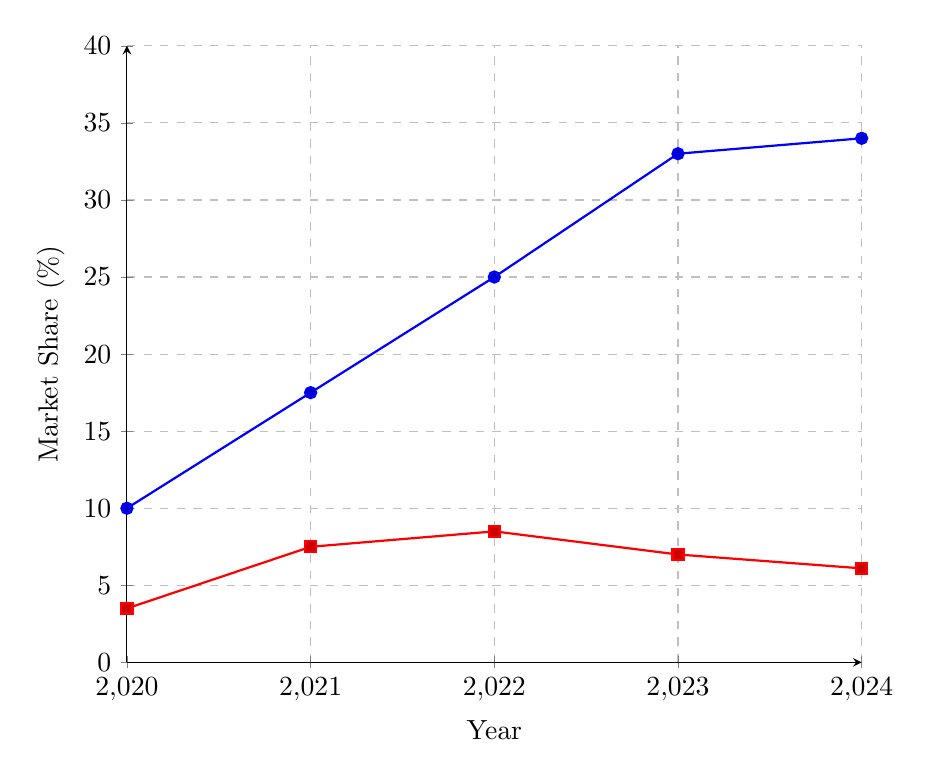
\begin{tikzpicture}
\begin{axis}[
    my_style,
    xlabel={Year},
    ylabel={Market Share (\%)},
    xtick={2020,2021,2022,2023,2024},
    ymin=0, ymax=40,
    legend columns=2,
    legend to name=legend2
]
\addplot+[mark=*, color=blue, thick] coordinates {
    (2020,10)
    (2021,17.5)
    (2022,25)
    (2023,33)
    (2024,34)
};
\addplot+[mark=square*, color=red, thick] coordinates {
    (2020,3.5)
    (2021,7.5)
    (2022,8.5)
    (2023,7)
    (2024,6.1)
};
\legend{BYD, Tesla}
\end{axis}
\end{tikzpicture}
\caption{Market Share in China NEV Segment: BYD vs. Tesla (2020--2024)}
\label{fig:china_marketshare}
\end{figure}

BYD's market share in China's NEV segment grew from a modest 10\% in 2020 to 32--36\% in 2024, driven by a mix of BEVs and PHEVs \citep{cnn2025, autovista2025}. Tesla's market share peaked at 8--9\% in 2022 but declined to about 6.1\% in 2024, despite record sales volumes, reflecting intensifying competition \citep{cnevpost2025, cnn2025}. BYD's total vehicle sales in China in 2024 reached approximately 4.1 million units, with BEVs accounting for about 1.76 million and PHEVs for 2.5 million \citep{tridens2025}. Tesla sold around 659,000 vehicles in China in 2024, primarily BEVs, with the Model 3 and Model Y as the main drivers \citep{autovista2025}.

\subsection{Global Production and Sales Volumes}

\begin{table}[ht]
\centering
\caption{Global Sales and Production: BYD vs. Tesla (2020--2024)}
\label{tab:global_sales}
\begin{tabularx}{\textwidth}{l l l l l}
\toprule
Year & BYD Global Sales & BYD BEV Sales & BYD PHEV Sales & Tesla Global BEV Sales \\
\midrule
2020 & 394,608 & 150,000 & 244,000 & 500,000 \\
2021 & 1,000,000 & 600,000 & 400,000 & 930,000 \\
2022 & 1,600,000 & 900,000 & 700,000 & 1,300,000 \\
2023 & 3,024,417 & 1,600,000 & 1,400,000 & 1,850,000 \\
2024 & 4,272,145 & 1,764,992 & 2,485,378 & 1,789,226 \\
\bottomrule
\end{tabularx}
\end{table}

\begin{figure}[ht]
\centering
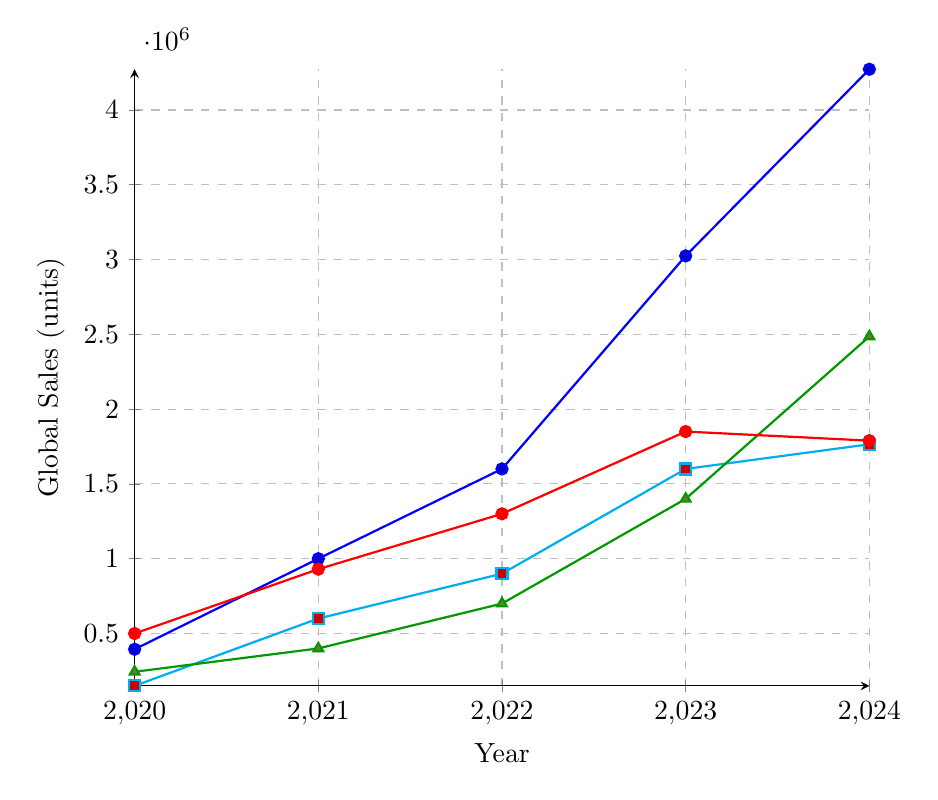
\begin{tikzpicture}
\begin{axis}[
    my_style,
    xlabel={Year},
    ylabel={Global Sales (units)},
    xtick={2020,2021,2022,2023,2024},
    legend columns=3,
    legend to name=legend3
]
\addplot+[mark=*, color=blue, thick] coordinates {
    (2020,394608)
    (2021,1000000)
    (2022,1600000)
    (2023,3024417)
    (2024,4272145)
};
\addplot+[mark=square*, color=cyan, thick] coordinates {
    (2020,150000)
    (2021,600000)
    (2022,900000)
    (2023,1600000)
    (2024,1764992)
};
\addplot+[mark=triangle*, color=green!60!black, thick] coordinates {
    (2020,244000)
    (2021,400000)
    (2022,700000)
    (2023,1400000)
    (2024,2485378)
};
\addplot+[mark=*, color=red, thick] coordinates {
    (2020,500000)
    (2021,930000)
    (2022,1300000)
    (2023,1850000)
    (2024,1789226)
};
\legend{BYD Total, BYD BEV, BYD PHEV, Tesla BEV}
\end{axis}
\end{tikzpicture}
\caption{Global Sales Volumes: BYD (Total, BEV, PHEV) and Tesla (BEV) (2020--2024)}
\label{fig:global_sales}
\end{figure}

BYD's global sales more than doubled from 2020 to 2024, with a 41.3\% increase in 2024 alone, driven by PHEV growth of over 70\% \citep{bestcars2024}. Tesla's global BEV sales peaked in 2023 at about 1.85 million units but declined slightly in 2024 to 1.79 million units \citep{insideevs2024}. In 2024, BYD surpassed Tesla in total EV production, producing 1,777,965 EVs compared to Tesla's 1,774,442 units, marking a pivotal shift in global EV manufacturing leadership \citep{statista2024}.

\section{Significant Trends and Events Affecting Market Positions}

\subsection{BYD's Strategic Focus and Expansion}

BYD's aggressive expansion in PHEVs, which accounted for over half of its 2024 sales, allowed it to capture a broader consumer base, especially in China where hybrids gained market share from 33.3\% in 2023 to 43.4\% in 2024 \citep{autovista2025, tridens2025}. BYD's pricing strategy, with models starting at around \$10,000, and technological innovations such as the Blade Battery and ultra-fast charging (5 minutes for 400 km), have been key differentiators \citep{scmp2024, cnn2025}.

\subsection{Tesla's Regulatory and Competitive Challenges}

Tesla faced regulatory delays for its Full Self-Driving (FSD) system in China, limiting its competitive edge in autonomous driving features. Its limited model lineup and higher price points constrained market share growth amid rising competition from domestic brands \citep{cnn2025, investors2025}. Tesla's market share declined from 7--8\% in 2021--2022 to about 6.1\% in 2024, despite record sales volumes \citep{cnevpost2025}.

\subsection{Price War and Market Dynamics}

In 2025, BYD launched a price war in China, offering 10--30\% discounts on EVs, leveraging its vertical integration and cost advantages. Tesla responded with price adjustments but struggled to match BYD's breadth and pricing flexibility \citep{investors2025}.

\subsection{Government Policy Impacts}

China's NEV subsidies (2020--2022), license plate advantages, and cash-for-clunkers programs favored BYD's growth. Conversely, U.S. policies like the Inflation Reduction Act (2022) favored Tesla's domestic production but limited BYD's U.S. market access due to tariffs and import restrictions \citep{techresearchonline2024, ielp2024}.

\section{Financial Performance Comparison (2024)}

\begin{table}[ht]
\centering
\caption{Financial Performance: BYD vs. Tesla (2024)}
\label{tab:financials}
\begin{tabularx}{\textwidth}{l l l}
\toprule
Metric & BYD (2024) & Tesla (2024) \\
\midrule
Revenue & \textasciitilde\$107 billion (777 billion yuan) & \$97.7 billion \\
Net Profit & $>$40 billion yuan (\textasciitilde\$6 billion) & \$7.1 billion \\
Market Cap (May 2025) & \$162.3 billion & \$1.09 trillion \\
Q1 2025 Net Income & \$1.26 billion (up 100\%) & \$934 million (down 40\%) \\
\bottomrule
\end{tabularx}
\end{table}

BYD's revenue and net profit in 2024 surpassed Tesla's, reflecting its dominant sales volume and diversified product portfolio \citep{cnn2025, investors2025}. However, Tesla's market capitalization remains substantially higher, reflecting investor confidence in its technology and global brand despite recent sales challenges \citep{investors2025}.

\section{Comparative Analysis: Strategy, Product, and Technology}

\begin{table}[ht]
\centering
\caption{Comparative Analysis: BYD vs. Tesla (2024)}
\label{tab:comparison}
\begin{tabularx}{\textwidth}{l l l}
\toprule
Aspect & BYD & Tesla \\
\midrule
Market Share (China 2024) & 32--36\% (NEV market) & 6.1--6.2\% (NEV market) \\
Sales Volume (China 2024) & \textasciitilde4.1 million vehicles (BEV + PHEV) & \textasciitilde659,000 vehicles (mostly BEV) \\
Global BEV Sales (2024) & 1.76 million BEVs + 2.5 million PHEVs & 1.79 million BEVs \\
Product Portfolio & Broad: affordable to premium, BEVs + PHEVs & Focused: premium BEVs (Model 3, Y, Cybertruck) \\
Pricing Strategy & Aggressive, price war, models from \textasciitilde\$10,000 & Premium pricing, limited discounts \\
Technology & Blade Battery, ultra-fast charging, advanced driver-assist included & 4680 battery cells, FSD (pending China), slower charging \\
Manufacturing & Concentrated in China, vertical integration & Gigafactories in US, China, Germany, expanding \\
Financials (2024) & Revenue \$107B, net profit $>$\$6B & Revenue \$97.7B, net profit \$7.1B \\
Market Cap (2025) & \$162.3 billion & \$1.09 trillion \\
Growth Trends & Rapid growth, expanding global footprint & Slower growth, facing competition and regulatory challenges \\
\bottomrule
\end{tabularx}
\end{table}

BYD's strategy centers on product diversity, affordability, and rapid innovation, enabling it to capture a broad market segment. Tesla, while maintaining a technological edge in autonomy and battery technology, faces challenges in model variety and pricing competitiveness in China \citep{teslarati2025, scmp2024, cnn2025}.

\section{Discussion: Key Drivers and Policy Implications}

\subsection{Product and Technology Innovation}

BYD's introduction of the Blade Battery, ultra-fast charging, and advanced driver-assistance systems at no extra cost have been critical in attracting Chinese consumers \citep{cnn2025, scmp2024}. Tesla's FSD and 4680 battery cells remain technological benchmarks, but regulatory delays and higher costs have limited their impact in China \citep{investors2025}.

\subsection{Government Policy and Market Access}

Chinese government support, including over \$230 billion in subsidies, has been instrumental in BYD's rise \citep{time2024}. U.S. tariffs and the Inflation Reduction Act have constrained BYD's access to the U.S. market, while Tesla has benefited from U.S. policy but faces headwinds in China \citep{ielp2024, techresearchonline2024}.

\subsection{Consumer Reception and Brand Dynamics}

BYD's broad product range and affordability have resonated with Chinese consumers, while Tesla's brand preference declined from 22\% to 18\% among Chinese buyers between 2023 and 2024 \citep{scmp2024}. BYD's ability to capitalize on Tesla's political controversies and shifting consumer sentiment has further strengthened its position.

\section{Conclusions and Future Outlook}

BYD's rapid ascent in the Chinese EV market from 2020 to 2024 reflects a strategic combination of diversified product offerings, aggressive pricing, vertical integration, and alignment with government policies. Its dominance in both BEV and PHEV segments, coupled with technological innovations, has enabled BYD to surpass Tesla in market share and sales volume in China by 2024 \citep{cnn2025, statista2024}.

Tesla remains a formidable competitor with a strong global brand and technological leadership, but faces challenges in China due to regulatory delays, limited model variety, and pricing pressures \citep{investors2025, cnevpost2025}. Looking ahead, BYD is expected to continue expanding its market share in China and internationally, supported by new manufacturing plants and ongoing product innovation \citep{investors2025, gasgoo2024}. Tesla's plans to introduce more affordable models and expand autonomous services may help regain momentum, but it faces stiff competition from BYD and other Chinese manufacturers \citep{teslarati2025}.

The evolution of China's EV market underscores the importance of product diversity, pricing strategy, and government policy alignment. BYD's rise challenges Tesla's global leadership and signals a broader shift toward Chinese dominance in the EV industry, with implications for global supply chains, technology development, and competitive strategies.

\begin{filecontents*}{references.bib}
@online{cnn2025,
  author = {CNN},
  title = {Chinese EV titan BYD annual sales hit \$100 billion eclipsing rival Tesla},
  year = {2025},
  url = {https://www.cnn.com/2025/03/25/cars/china-byd-annual-sales-pass-tesla-intl-hnk},
  note = {Accessed: 2025-07-01}
}
@online{autovista2025,
  author = {Autovista24},
  title = {Which brand won the battle for China’s EV market?},
  year = {2025},
  url = {https://autovista24.autovistagroup.com/news/which-brand-won-the-battle-for-chinas-ev-market},
  note = {Accessed: 2025-07-01}
}
@online{tridens2025,
  author = {Tridens Technology},
  title = {BYD Sales by Model and Country Statistics (Feb 2025)},
  year = {2025},
  url = {https://tridenstechnology.com/byd-sales-statistics},
  note = {Accessed: 2025-07-01}
}
@online{cnevpost2025,
  author = {CNEVPost},
  title = {Automakers' share of China NEV market in May: BYD No. 1 with 28.5\%, Tesla No. 8 with 3.8\%},
  year = {2025},
  url = {https://cnevpost.com/2025/06/10/automakers-share-china-nev-market-may-2025},
  note = {Accessed: 2025-07-01}
}
@online{bestcars2024,
  author = {Best-Selling Cars},
  title = {2024 (Full Year) Global: BYD Worldwide Car Sales and Productions},
  year = {2024},
  url = {https://www.best-selling-cars.com/brands/2024-full-year-global-byd-worldwide-car-sales-and-productions},
  note = {Accessed: 2025-07-01}
}
@online{insideevs2024,
  author = {InsideEVs},
  title = {China's BYD Was The Top EV Maker In 2024, Beating Tesla},
  year = {2024},
  url = {https://insideevs.com/news/746064/byd-beats-tesla-ev-production},
  note = {Accessed: 2025-07-01}
}
@online{statista2024,
  author = {Statista},
  title = {Infographic: BYD Pulls Ahead of Tesla to Become Largest EV Maker},
  year = {2024},
  url = {https://www.statista.com/chart/33709/tesla-byd-electric-vehicle-production},
  note = {Accessed: 2025-07-01}
}
@online{autovista2025b,
  author = {Autovista24},
  title = {Which brand won the battle for China’s EV market?},
  year = {2025},
  url = {https://autovista24.autovistagroup.com/news/which-brand-won-the-battle-for-chinas-ev-market},
  note = {Accessed: 2025-07-01}
}
@online{investors2025,
  author = {Investors.com},
  title = {Tesla Vs. BYD As Of May 26: TSLA Has New Buy Point; BYD Launches Price War},
  year = {2025},
  url = {https://www.investors.com/news/tesla-vs-byd-ev-sales-robotaxis},
  note = {Accessed: 2025-07-01}
}
@online{techresearchonline2024,
  author = {TechResearchOnline},
  title = {Tesla vs. BYD: Who’s Winning the Global EV Race?},
  year = {2024},
  url = {https://techresearchonline.com/blog/tesla-vs-byd-the-global-ev-race},
  note = {Accessed: 2025-07-01}
}
@online{ielp2024,
  author = {IELP},
  title = {Guest Post: Commerce Department Regulations on “Connected” Vehicles},
  year = {2024},
  url = {https://ielp.worldtradelaw.net/2024/10/guest-post-commerce-department-regulations-on-connected-vehicles-potential-impacts-on-chinese-mexica.html},
  note = {Accessed: 2025-07-01}
}
@online{time2024,
  author = {Time},
  title = {The Shift East: How China’s EV Boom Powers Its Tech Rise},
  year = {2024},
  url = {https://time.com/7288660/shift-east-china-electric-vehicles-economy-technology-trump-tariffs-ai},
  note = {Accessed: 2025-07-01}
}
@online{sciencedirect2023,
  author = {ScienceDirect},
  title = {Competition and welfare effects of introducing new products into the new energy vehicle market: Empirical evidence from Tesla’s entry into the Chinese market},
  year = {2023},
  url = {https://www.sciencedirect.com/science/article/abs/pii/S0965856423001507},
  note = {Accessed: 2025-07-01}
}
@online{gasgoo2024,
  author = {Gasgoo},
  title = {Top stories of BYD in 2024},
  year = {2024},
  url = {https://autonews.gasgoo.com/china_news/70035802.html},
  note = {Accessed: 2025-07-01}
}
@online{teslarati2025,
  author = {TeslaRati},
  title = {BYD to overtake Tesla in BEV sales this 2025: Counterpoint Research},
  year = {2025},
  url = {https://www.teslarati.com/byd-to-overtake-tesla-bev-sales-2025-counterpoint},
  note = {Accessed: 2025-07-01}
}
@online{scmp2024,
  author = {South China Morning Post},
  title = {BYD launches a 'Model 3 killer' EV in China for half the price of Tesla's top seller},
  year = {2024},
  url = {https://www.scmp.com/business/china-evs/article/3303614/chinas-byd-launches-ev-rival-teslas-top-seller-around-half-price},
  note = {Accessed: 2025-07-01}
}
\end{filecontents*}

\bibliographystyle{unsrt}
\bibliography{references}

\end{document}